%%%%%%%%%%%%%%%%%%%%%%%%%%%%%%%%%%%%%%%%%%%%%%%%%%%%%%%%%%%%%%%%%%%%%%%%%%%%
% AGUtmpl.tex: this template file is for articles formatted with LaTeX2e,
% Modified September 2012
%
% This template includes commands and instructions
% given in the order necessary to produce a final output that will
% satisfy AGU requirements.
%
% PLEASE DO NOT USE YOUR OWN MACROS
% DO NOT USE \newcommand, \renewcommand, or \def.
%
% FOR FIGURES, DO NOT USE \psfrag or \subfigure.
%
%%%%%%%%%%%%%%%%%%%%%%%%%%%%%%%%%%%%%%%%%%%%%%%%%%%%%%%%%%%%%%%%%%%%%%%%%%%%
%
% All questions should be e-mailed to latex@agu.org.
%
%%%%%%%%%%%%%%%%%%%%%%%%%%%%%%%%%%%%%%%%%%%%%%%%%%%%%%%%%%%%%%%%%%%%%%%%%%%%
%
% Step 1: Set the \documentclass
%
% There are two options for article format: two column (default)
% and draft.
%
% PLEASE USE THE DRAFT OPTION TO SUBMIT YOUR PAPERS.
% The draft option produces double spaced output.
%
% Choose the journal abbreviation for the journal you are
% submitting to:

% jgrga JOURNAL OF GEOPHYSICAL RESEARCH
% gbc   GLOBAL BIOCHEMICAL CYCLES
% grl   GEOPHYSICAL RESEARCH LETTERS
% pal   PALEOCEANOGRAPHY
% ras   RADIO SCIENCE
% rog   REVIEWS OF GEOPHYSICS (if you encounter problems with this class file, use jgrga instead)
% tec   TECTONICS
% wrr   WATER RESOURCES RESEARCH
% gc    GEOCHEMISTRY, GEOPHYSICS, GEOSYSTEMS
% sw    SPACE WEATHER
%
% For JOURNAL OF ADVANCES IN MODELING EARTH SYSTEMS, use jgrga.
%
%
% (If you are submitting to a journal other than jgrga,
% substitute the initials of the journal for "jgrga" below.)

\documentclass[draft,jgrga]{agutex}

%%%%%%%%%%%%%%%%%%%%%%%%%%%%%%%%%%%%%%%%%%%%%%%%%%%%%%%%%%%%%%%%%%%%%%%%%
% OPTIONAL:
% To produce a two-columned version:
%\documentclass[jgrga]{AGUTeX}

% Two-columned format can be used to estimate the number of pages
% for the final published PDF.

% PLEASE USE THE DRAFT OPTION TO SUBMIT YOUR PAPERS.
%%%%%%%%%%%%%%%%%%%%%%%%%%%%%%%%%%%%%%%%%%%%%%%%%%%%%%%%%%%%%%%%%%%%%%%%%
% OPTIONAL:
% To create numbered lines:

% If you don't already have lineno.sty, you can download it from
% http://www.ctan.org/tex-archive/macros/latex/contrib/ednotes/
% (or search the internet for lineno.sty ctan), available at TeX Archive Network (CTAN).
% Take care that you always use the latest version.

% To activate the commands, uncomment \usepackage{lineno}
% and \linenumbers*[1]command, below:

\usepackage{lineno}
\linenumbers*[1]

%  To add line numbers to lines with equations:
% \begin{linenomath*}
%\begin{equation}
%\end{equation}
%\end{linenomath*}
%%%%%%%%%%%%%%%%%%%%%%%%%%%%%%%%%%%%%%%%%%%%%%%%%%%%%%%%%%%%%%%%%%%%%%%%%
% Figures and Tables
%
% When submitting articles through the GEMS system:
% COMMENT OUT ANY COMMANDS THAT INCLUDE GRAPHICS.
% (See FIGURES section near the end of the file.)
%
% DO NOT USE \psfrag or \subfigure commands.
%
%  Figures and tables should be placed AT THE END OF THE ARTICLE,
%  after the references.
%
%  Uncomment the following command to include .eps files
%  (comment out this line for draft format):
\usepackage{graphicx}
%
%  Uncomment the following command to allow illustrations to print
%   when using Draft:
%\setkeys{Gin}{draft=True}
%
% Substitute one of the following for [dvips] above
% if you are using a different driver program and want to
% proof your illustrations on your machine:
%
% [xdvi], [dvipdf], [dvipsone], [dviwindo], [emtex], [dviwin],
% [pctexps],  [pctexwin],  [pctexhp],  [pctex32], [truetex], [tcidvi],
% [oztex], [textures]
%
% See how to enter figures and tables at the end of the article, after
% references.
%
%%%%%%%%%% Start TeXmacs macros
\usepackage{amsmath,bbm}
\newcommand{\nonesep}{}
\newcommand{\tmem}[1]{{\em #1\/}}
\newcommand{\tmop}[1]{\ensuremath{\operatorname{#1}}}
\newcommand{\tmsamp}[1]{\textsf{#1}}
\newcommand{\tmstrong}[1]{\textbf{#1}}
\newcommand{\tmtextit}[1]{{\itshape{#1}}}
\newcommand{\parby}[2]{\ensuremath{\frac{\partial #1}{\partial #2}}}
\newcommand{\E}{\ensuremath{\vec{E}}}
\newcommand{\V}{\ensuremath{\vec{v}}}
\newcommand{\U}{\ensuremath{\vec{u}}}
\newcommand{\B}{\ensuremath{\vec{B}}}
\newcommand{\J}{\ensuremath{\vec{J}}}
\newcommand{\Vper}{\ensuremath{\vec{v}_{\perp}}}
\newcommand{\Vpara}{\ensuremath{\vec{v}_{\parallel}}}
\newcommand{\Uper}{\ensuremath{\vec{u}_{\perp}}}
\newcommand{\Upara}{\ensuremath{\vec{u}_{\parallel}}}
\newcommand{\X}{\ensuremath{\vec{x}}}
\newcommand{\DIV}{\ensuremath{\nabla \cdot}}
\newcommand{\CURL}{\ensuremath{\nabla \times}}
%%%%%%%%%% End TeXmacs macros
\usepackage{setspace}
%% ------------------------------------------------------------------------ %%
%
%  ENTER PREAMBLE
%
%% ------------------------------------------------------------------------ %%

% Author names in capital letters:
\authorrunninghead{WILTBERGER ET AL.}


% Shorter version of title entered in capital letters:
\titlerunninghead{Effects of AEH}

%Corresponding author mailing address and e-mail address:
%\authoraddr{Corresponding author: A. B. Smith,
%Department of Hydrology and Water Resources, University of
%Arizona, Harshbarger Building 11, Tucson, AZ 85721, USA.
%(a.b.smith@hwr.arizona.edu)}
\authoraddr{Corresponding author: M. Wiltberger,
National Center for Atmospheric Research,
High Altitude Observatory,
3080 Center Green,
Boulder, CO 80301
(wiltbemj@ucar.edu)}
\paperid{???}
\begin{document}

\def\oplus{O$^+$ }
\def\hplus{H$^+$ }
\def\heplus{He$^+$}
\def\nplus{N$^+$}
\def\dst{$D_{ST}$ }


%% ------------------------------------------------------------------------ %%
%
%  TITLE
%
%% ------------------------------------------------------------------------ %%


\title{Effects of Anomalous Electron Heating in simulations of the March 17, 2013 Geomagnetic Storm}
%
% e.g., \title{Terrestrial ring current:
% Origin, formation, and decay $\alpha\beta\Gamma\Delta$}
%

%% ------------------------------------------------------------------------ %%
%
%  AUTHORS AND AFFILIATIONS
%
%% ------------------------------------------------------------------------ %%


%Use \author{\altaffilmark{}} and \altaffiltext{}


% \altaffilmark will produce footnote;
% matching \altaffiltext will appear at bottom of page.

% \authors{A. B. Smith,\altaffilmark{1}
% Eric Brown,\altaffilmark{1,2} Rick Williams,\altaffilmark{3}
% John B. McDougall\altaffilmark{4}, and S. Visconti\altaffilmark{5}}

%\altaffiltext{1}{Department of Hydrology and Water Resources,
%University of Arizona, Tucson, Arizona, USA.}

%\altaffiltext{2}{Department of Geography, Ohio State University,
%Columbus, Ohio, USA.}

%\altaffiltext{3}{Department of Space Sciences, University of
%Michigan, Ann Arbor, Michigan, USA.}

%\altaffiltext{4}{Division of Hydrologic Sciences, Desert Research
%Institute, Reno, Nevada, USA.}

%\altaffiltext{5}{Dipartimento di Idraulica, Trasporti ed
%Infrastrutture Civili, Politecnico di Torino, Turin, Italy.}

\authors{M. Wiltberger, \altaffilmark{1}
V. Merkin, \altaffilmark{2}
B. Zhang,   \altaffilmark{1}
F. Toffletto,  \altaffilmark{3}
M. Oppenheim,  \altaffilmark{4}
W. Wang,  \altaffilmark{1}
J. G. Lyon, \altaffilmark{5}
J. Liu,  \altaffilmark{1}
and Y Dimant \altaffilmark{4}
}

\altaffiltext{1}
{High Altitude Observatory, National Center for Atmospheric Research,Boulder, Colorado, USA.}

\altaffiltext{2}{Applied Physics Laboratory, Johns Hopkins University, MD, USA.}

\altaffiltext{3}{Department of Physics and Astronomy, Rice University, TX, USA.}

\altaffiltext{4}{2Center for Space Physics, Boston University, Boston, Massachusetts, USA}

\altaffiltext{5}{Department of Physics and Astronomy, Dartmouth College,Hanover, NH, USA.}
%

%% ------------------------------------------------------------------------ %%
%
%  ABSTRACT
%
%% ------------------------------------------------------------------------ %%

% >> Do NOT include any \begin...\end commands within
% >> the body of the abstract.

\begin{abstract}
Examines the impacts of including Anomalous Electron Heating (AEH) in simulations of to the geomagnetic storm that occurred on 17 March 2013.   We see many cool things.

\end{abstract}

%% ------------------------------------------------------------------------ %%
%
%  BEGIN ARTICLE
%
%% ------------------------------------------------------------------------ %%

% The body of the article must start with a \begin{article} command
%
% \end{article} must follow the references section, before the figures
%  and tables.

\begin{article}

%% ------------------------------------------------------------------------ %%
%
%  TEXT
%
%% ------------------------------------------------------------------------ %%

\section{Introduction}

Here we will need to include a background 

\section{Simulation Setup}
\label{sec-model-sims}
This section discusses the simulation setup for the study.  Need to address how LFM-RCM works for situtaions with dipole tilt.  Need to discuss the implmentation of the AEH term.  And finally the setup for the 17 March 2013 event.

\subsection{LFM-RCM}

This section covers how LFM-RCM has been modified to work for dipole tilts.

\subsection{AEH Implementation}

Here we discuss how the AEH term has been included in the simulation.

\subsection{17 March 2013 Event}

Here we talk about the conditions  during the event

\begin{figure}
\noindent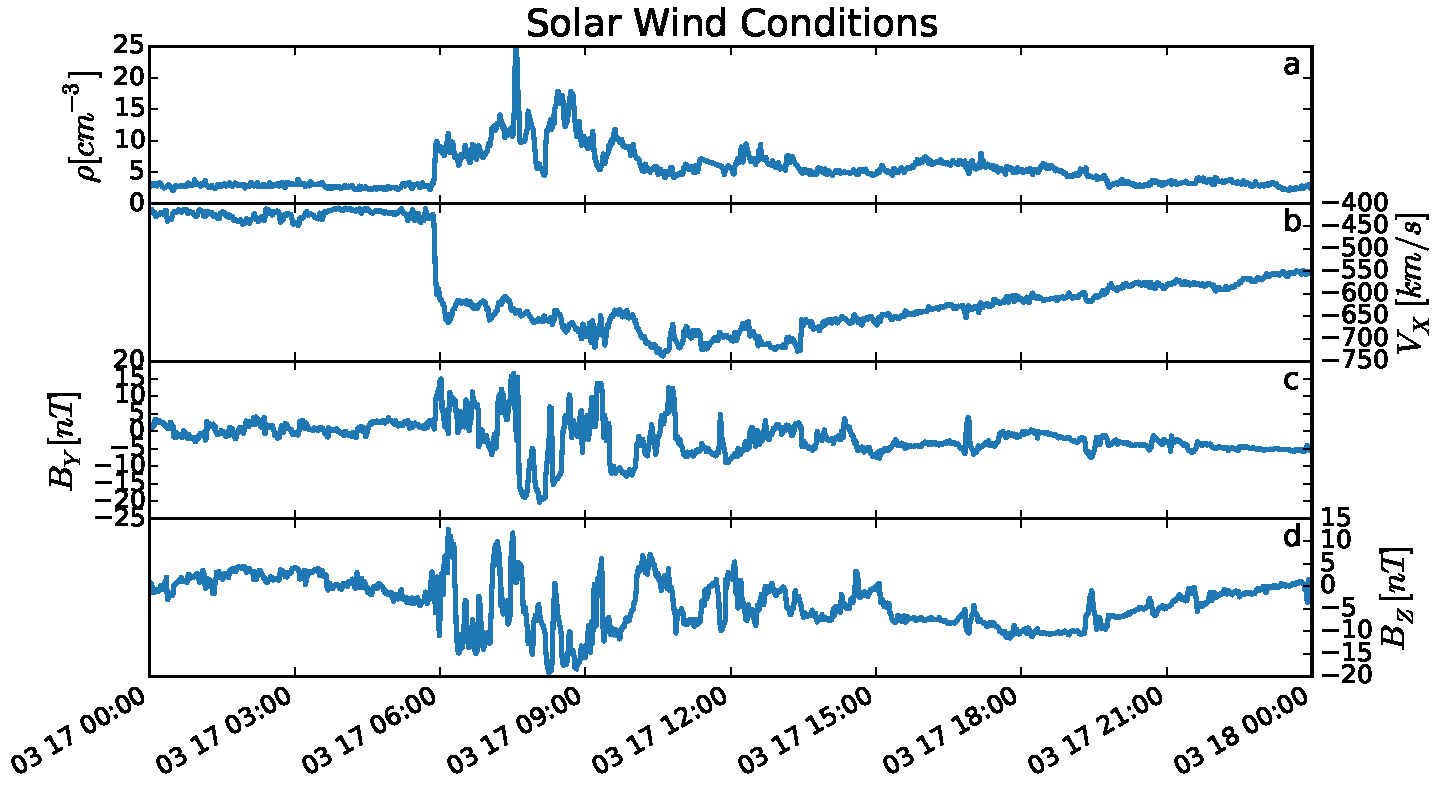
\includegraphics[width=20pc]{JGRPaper-SWFig.pdf}
\caption{\label{sw-fig} 
Solar wind and IMF conditions during the 17 March 2013 geomagnetic storm event.  Panel a) shows the number density, b) the $V_X$ in GSM coordinates.  The IMF GSM Y and Z values are plotted in panels c) and d) respectively.} 
\end{figure}

\section{Analysis of results}
\label{sec-analysis}
In this section we examine impact of the using AEH.

\subsection{Baseline versus AEH}
Possible figures include 

\begin{figure*}[t]
\noindent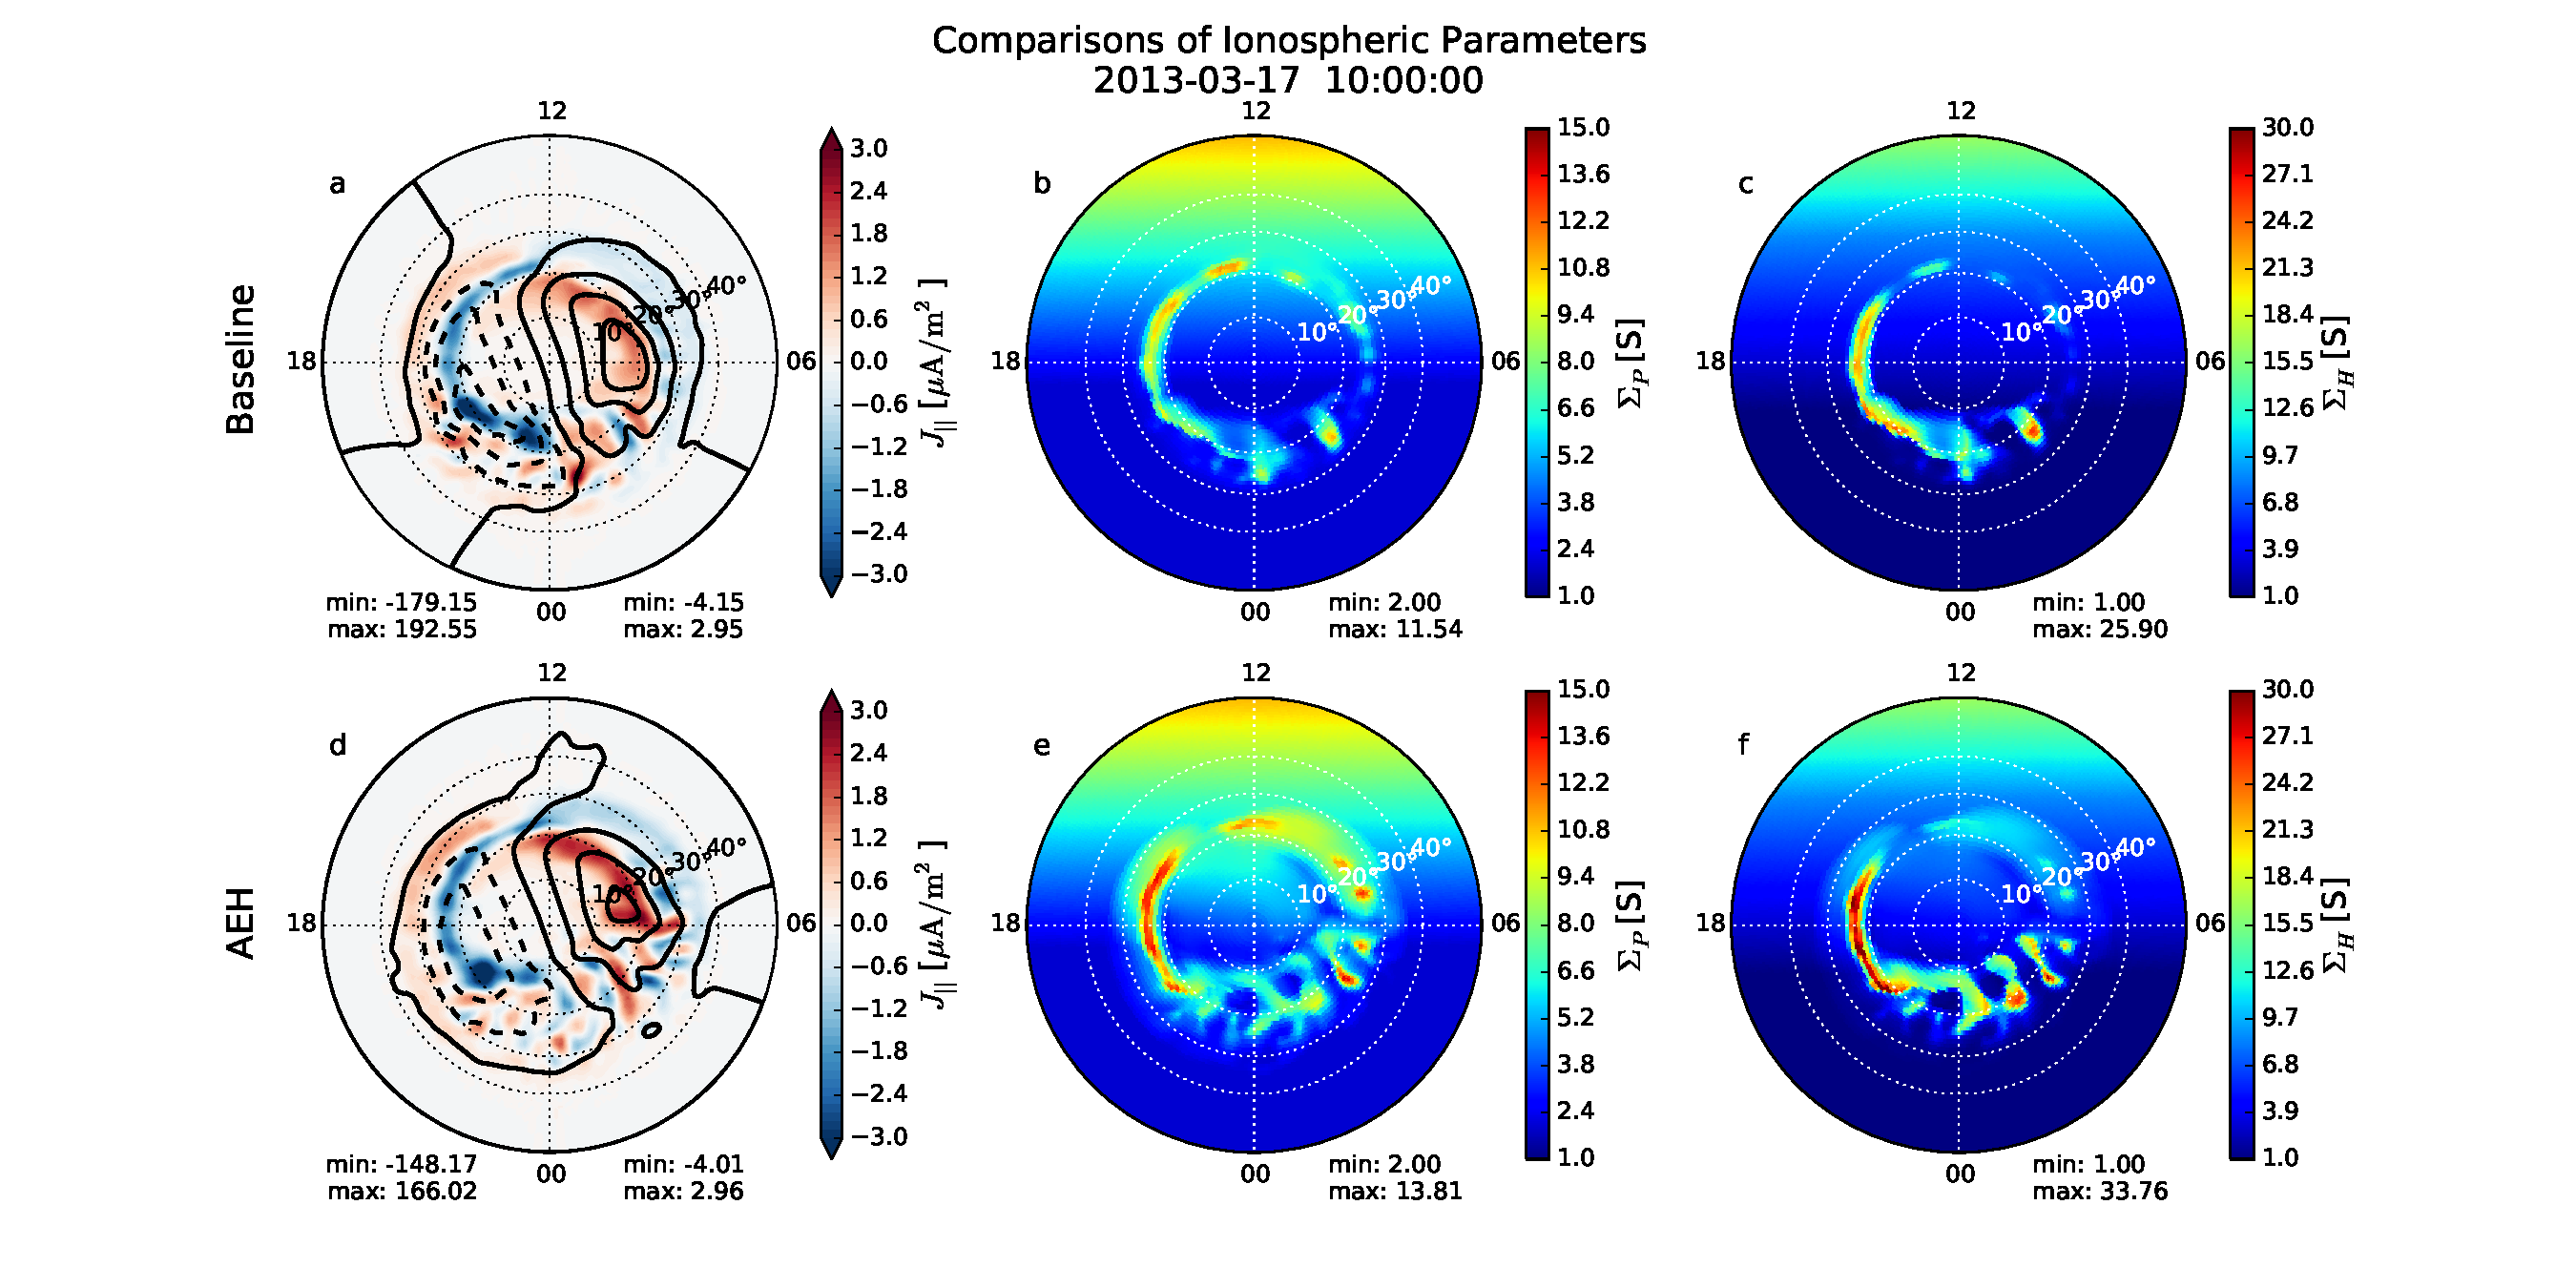
\includegraphics[width=39pc]{JGRPaper-IonPatterns.pdf}
\caption{\label{ion-comp-fig}
Comparison of FAC and CPCP as well as Pedersen and Hall conductivities for the Baseline and AEH simulations of the 17 March 2016 geomagnetic storm.  The top row (panels a-c) contains the results from the baseline simulation while the bottom row (panels d-f) contains the results of the simulation with the AEH enabled.  The first column (panels a and d) has the FAC in color with blue being upward and red being downward as well as the CPCP pattern with 20 kV contours.  The middle column (panels b and e) contains the Pedersen conductivity.  The last column (panels c and f) contains the Hall conductivity.  The colorbar for all conductivity plots is the same.}
\end{figure*}

\begin{figure}
\noindent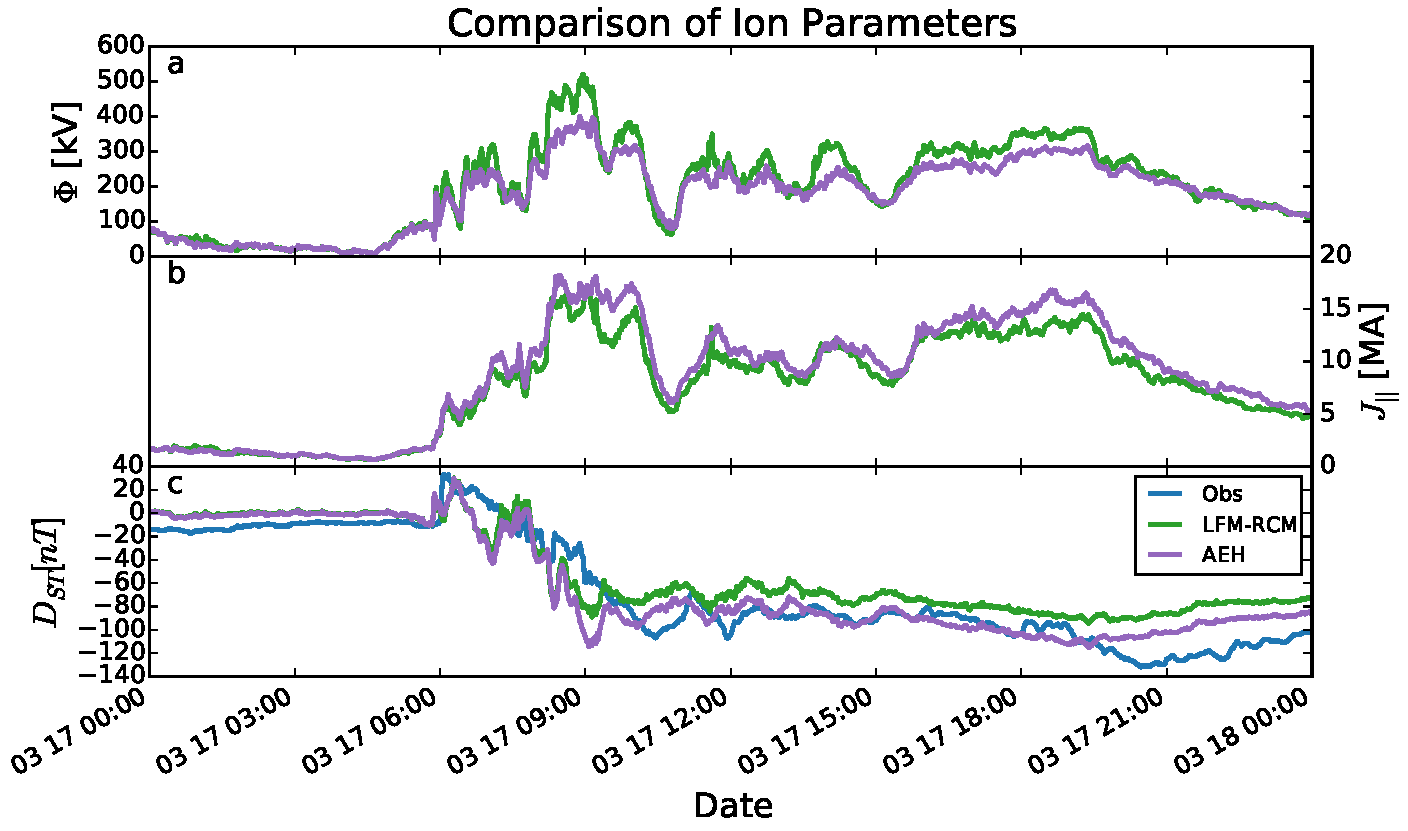
\includegraphics[width=20pc]{JGRPaper-IonFig.pdf}
\caption{\label{ts-fig} 
Comparison of the CPCP, FAC, and $D_{ST}$ time series for the storm event for the Northern hemisphere .  Panel a at the top shows the CPCP in kV.  The middle panel (b) has the integrated  FAC.  Panel c at the bottom has the $D_{ST}$ index.  In each panel the LFM-RCM results are shown with the green line, the AEH results with the purple line.  In the bottom panel the $D_{ST}$ obtained from CDAWeb is plotted in blue} 
\end{figure}

 \subsection{Comparison with DSMP}
 Here will discuss SAPs and the comparison with the DSMP results.
 
 \begin{figure*}[t]
\noindent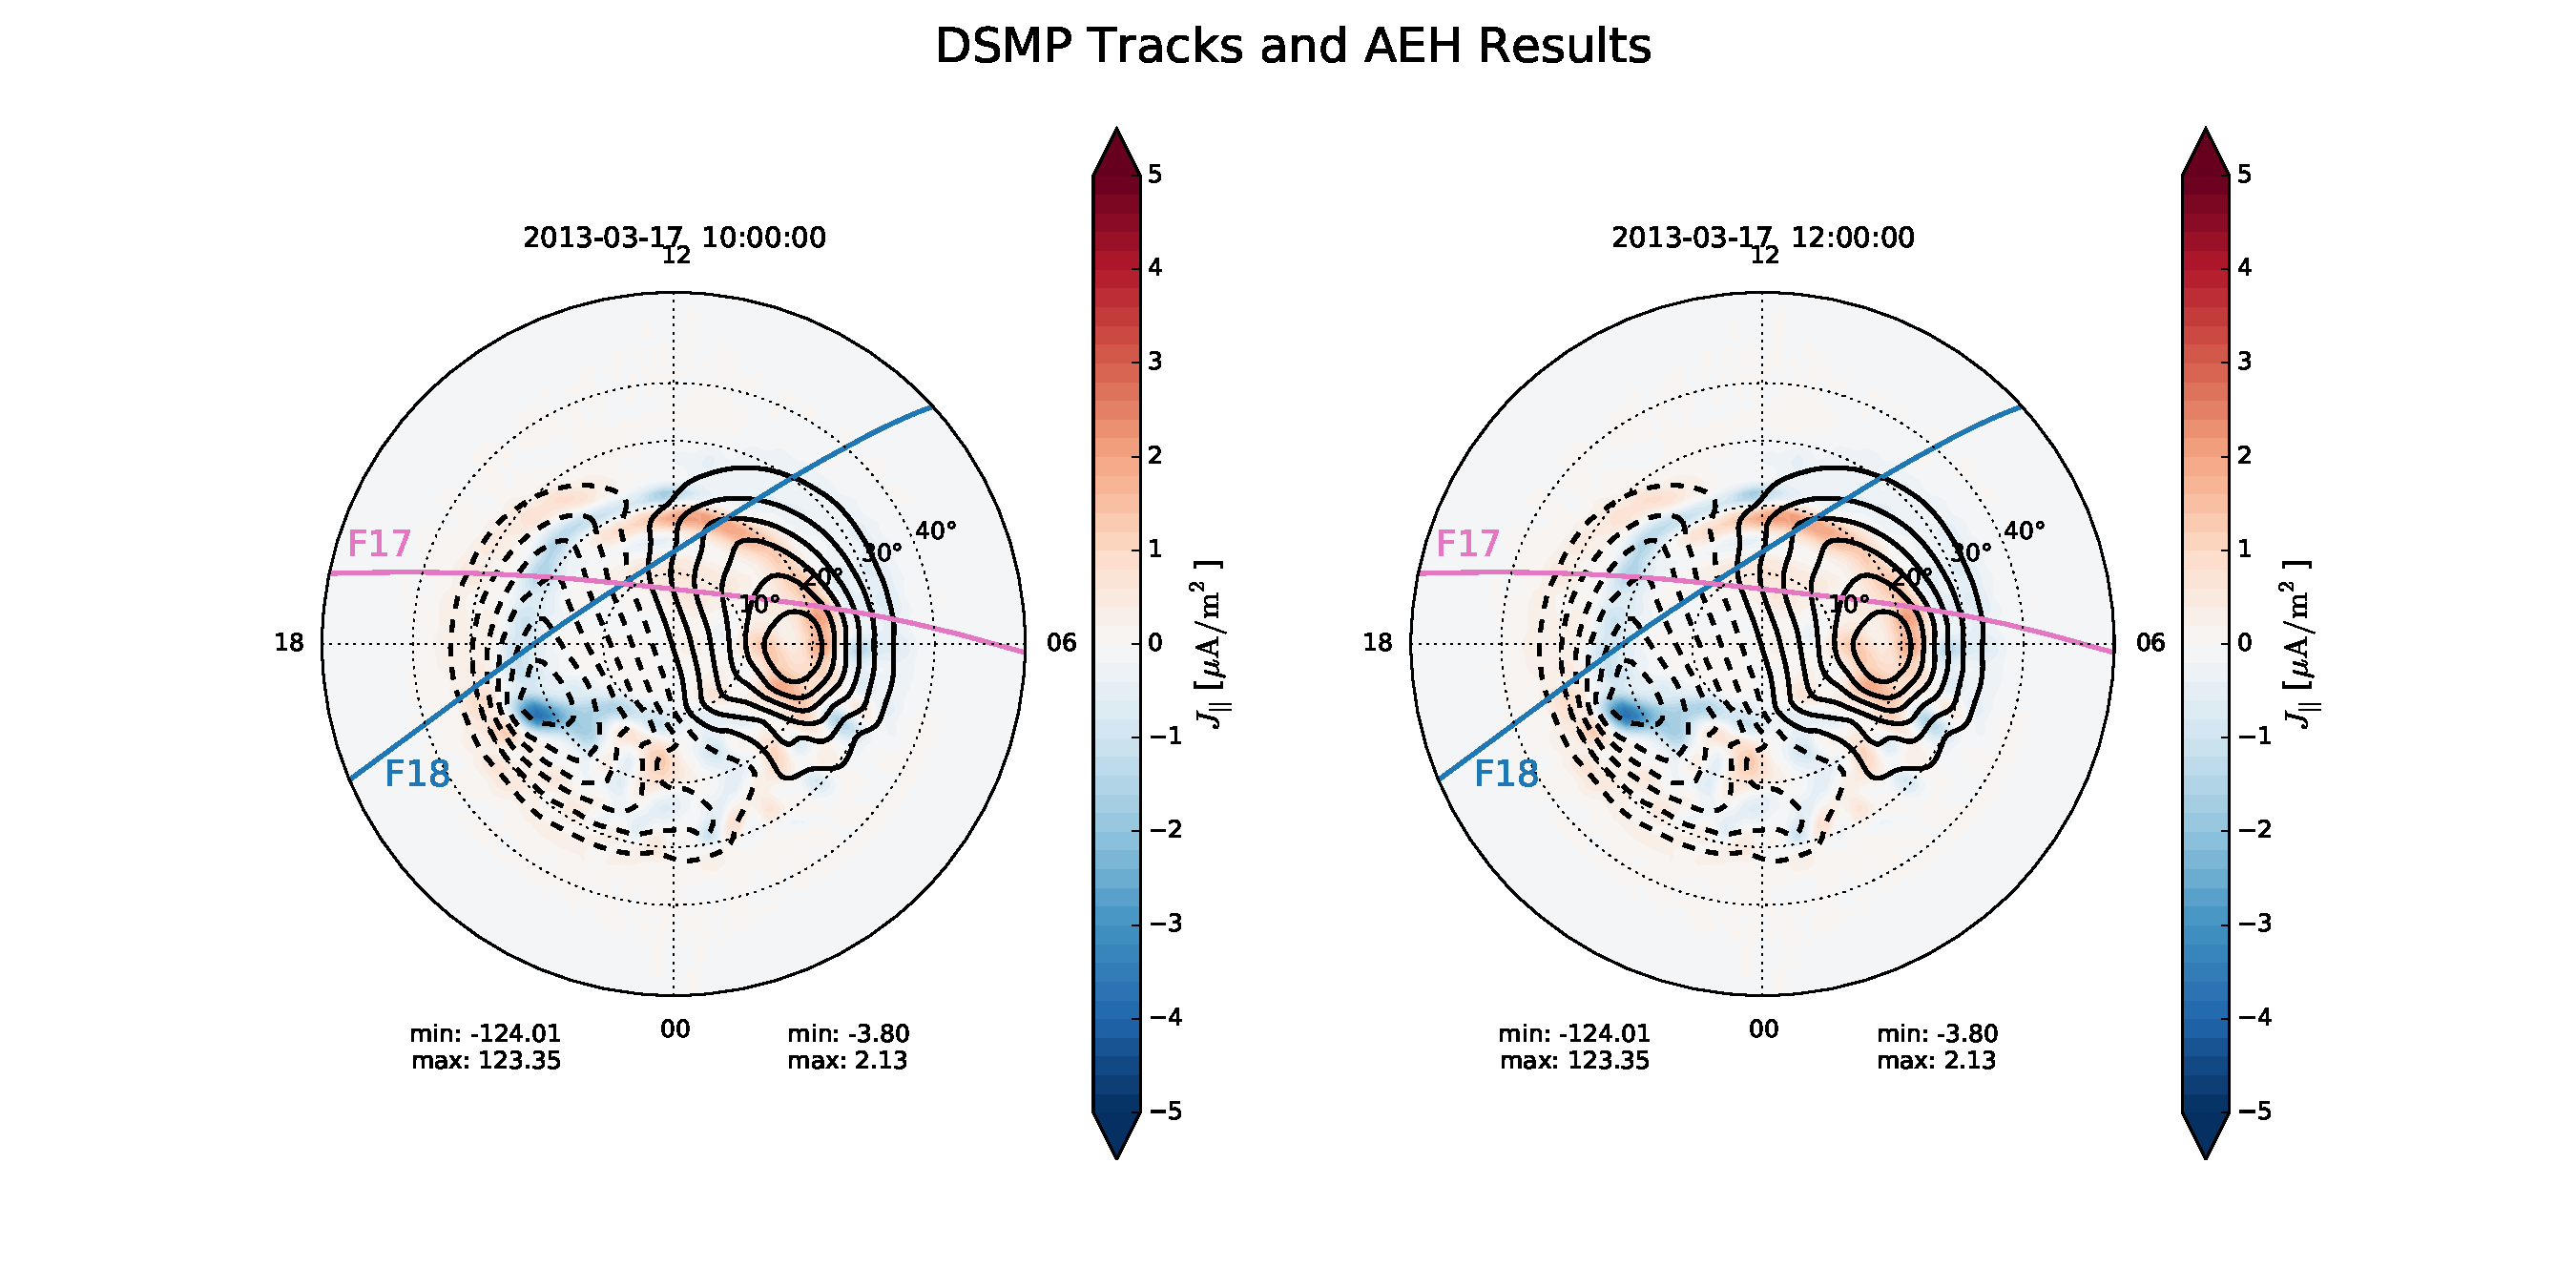
\includegraphics[width=39pc]{DMSPTraj.pdf}
\caption{\label{dmsptraj-fig}
DSMP F17 and F18 trajectories overlaid ontop of AEH FAC and CPCP patterns.  Panel a shows the F17 trajectory between 0945 and 1030 UT and the F18 trajectory beteween 1000 and 1045 UT overlaid on top of the AEH simulation results for 10:00UT.   Panel b shows the F17 trajectory between 1125 and 1210 UT and the F18 trajectory beteween 1145 and 1230 UT overlaid on top of the AEH simulation results for 12:00UT.  In each panel the F17 trajectory is pink and the F18 trajectory is blue.}
\end{figure*}

\begin{figure*}[t]
\noindent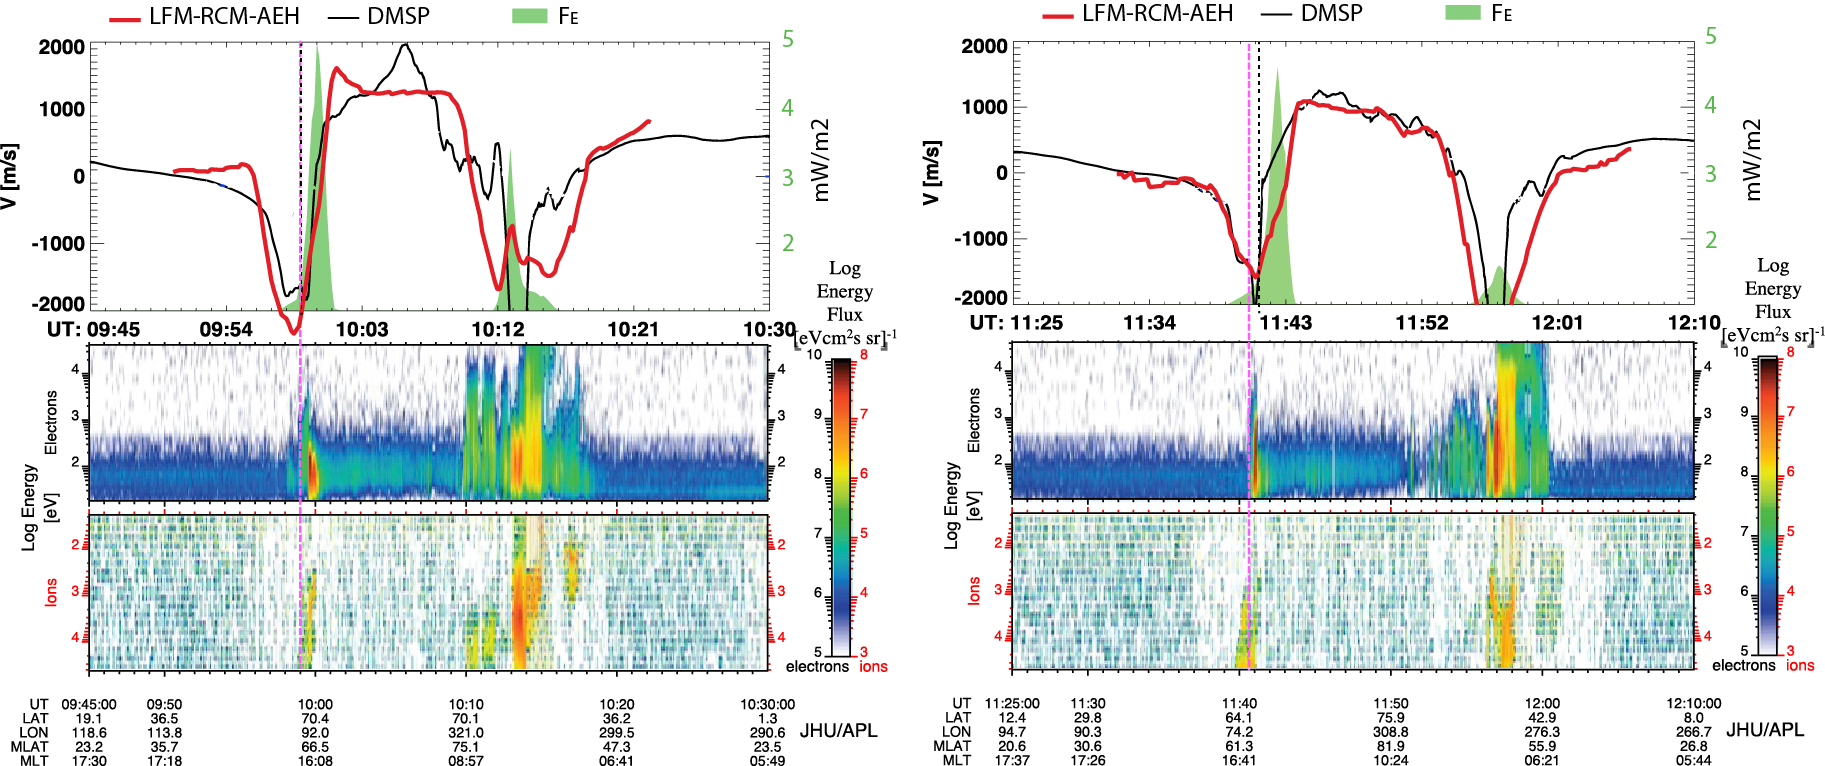
\includegraphics[width=39pc]{DMSP_F17_AEH_compare.png}
\caption{\label{f17-comp-fig}
Temporary Figure comparing DMSP F17 results. }
\end{figure*}

\begin{figure*}[t]
\noindent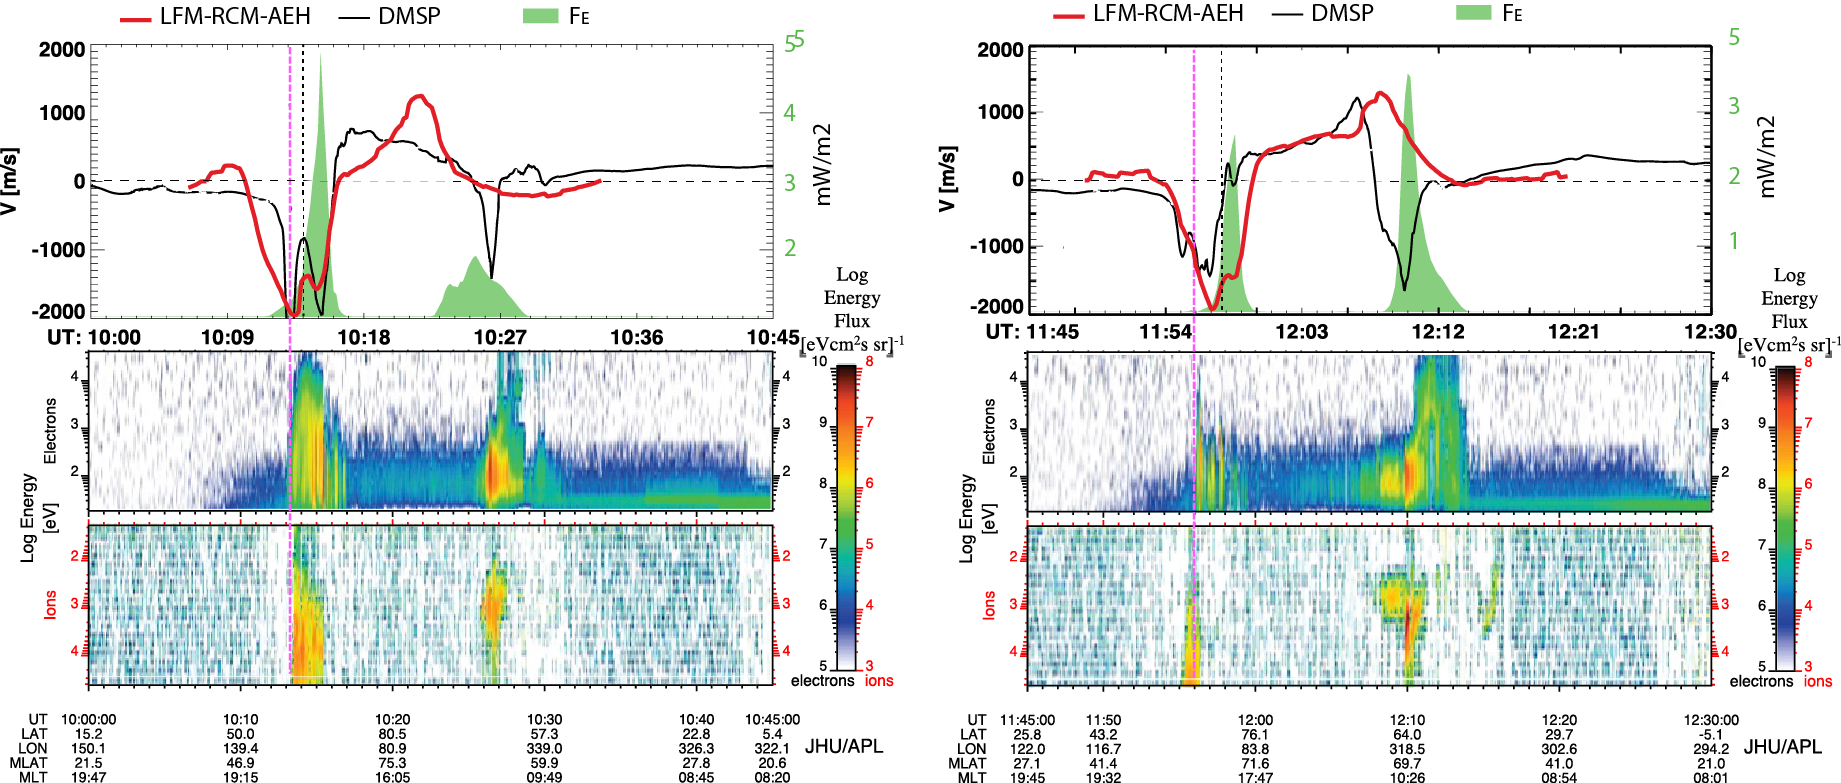
\includegraphics[width=39pc]{DMSP_F18_AEH_compare.png}
\caption{\label{f18-comp-fig}
Temporary Figure comparing DMSP F18 results}
\end{figure*}

 \subsection{Comparison with AMPERE}
 Here will discuss the results and compare them with AMPERE
 
\begin{figure*}[t]
\noindent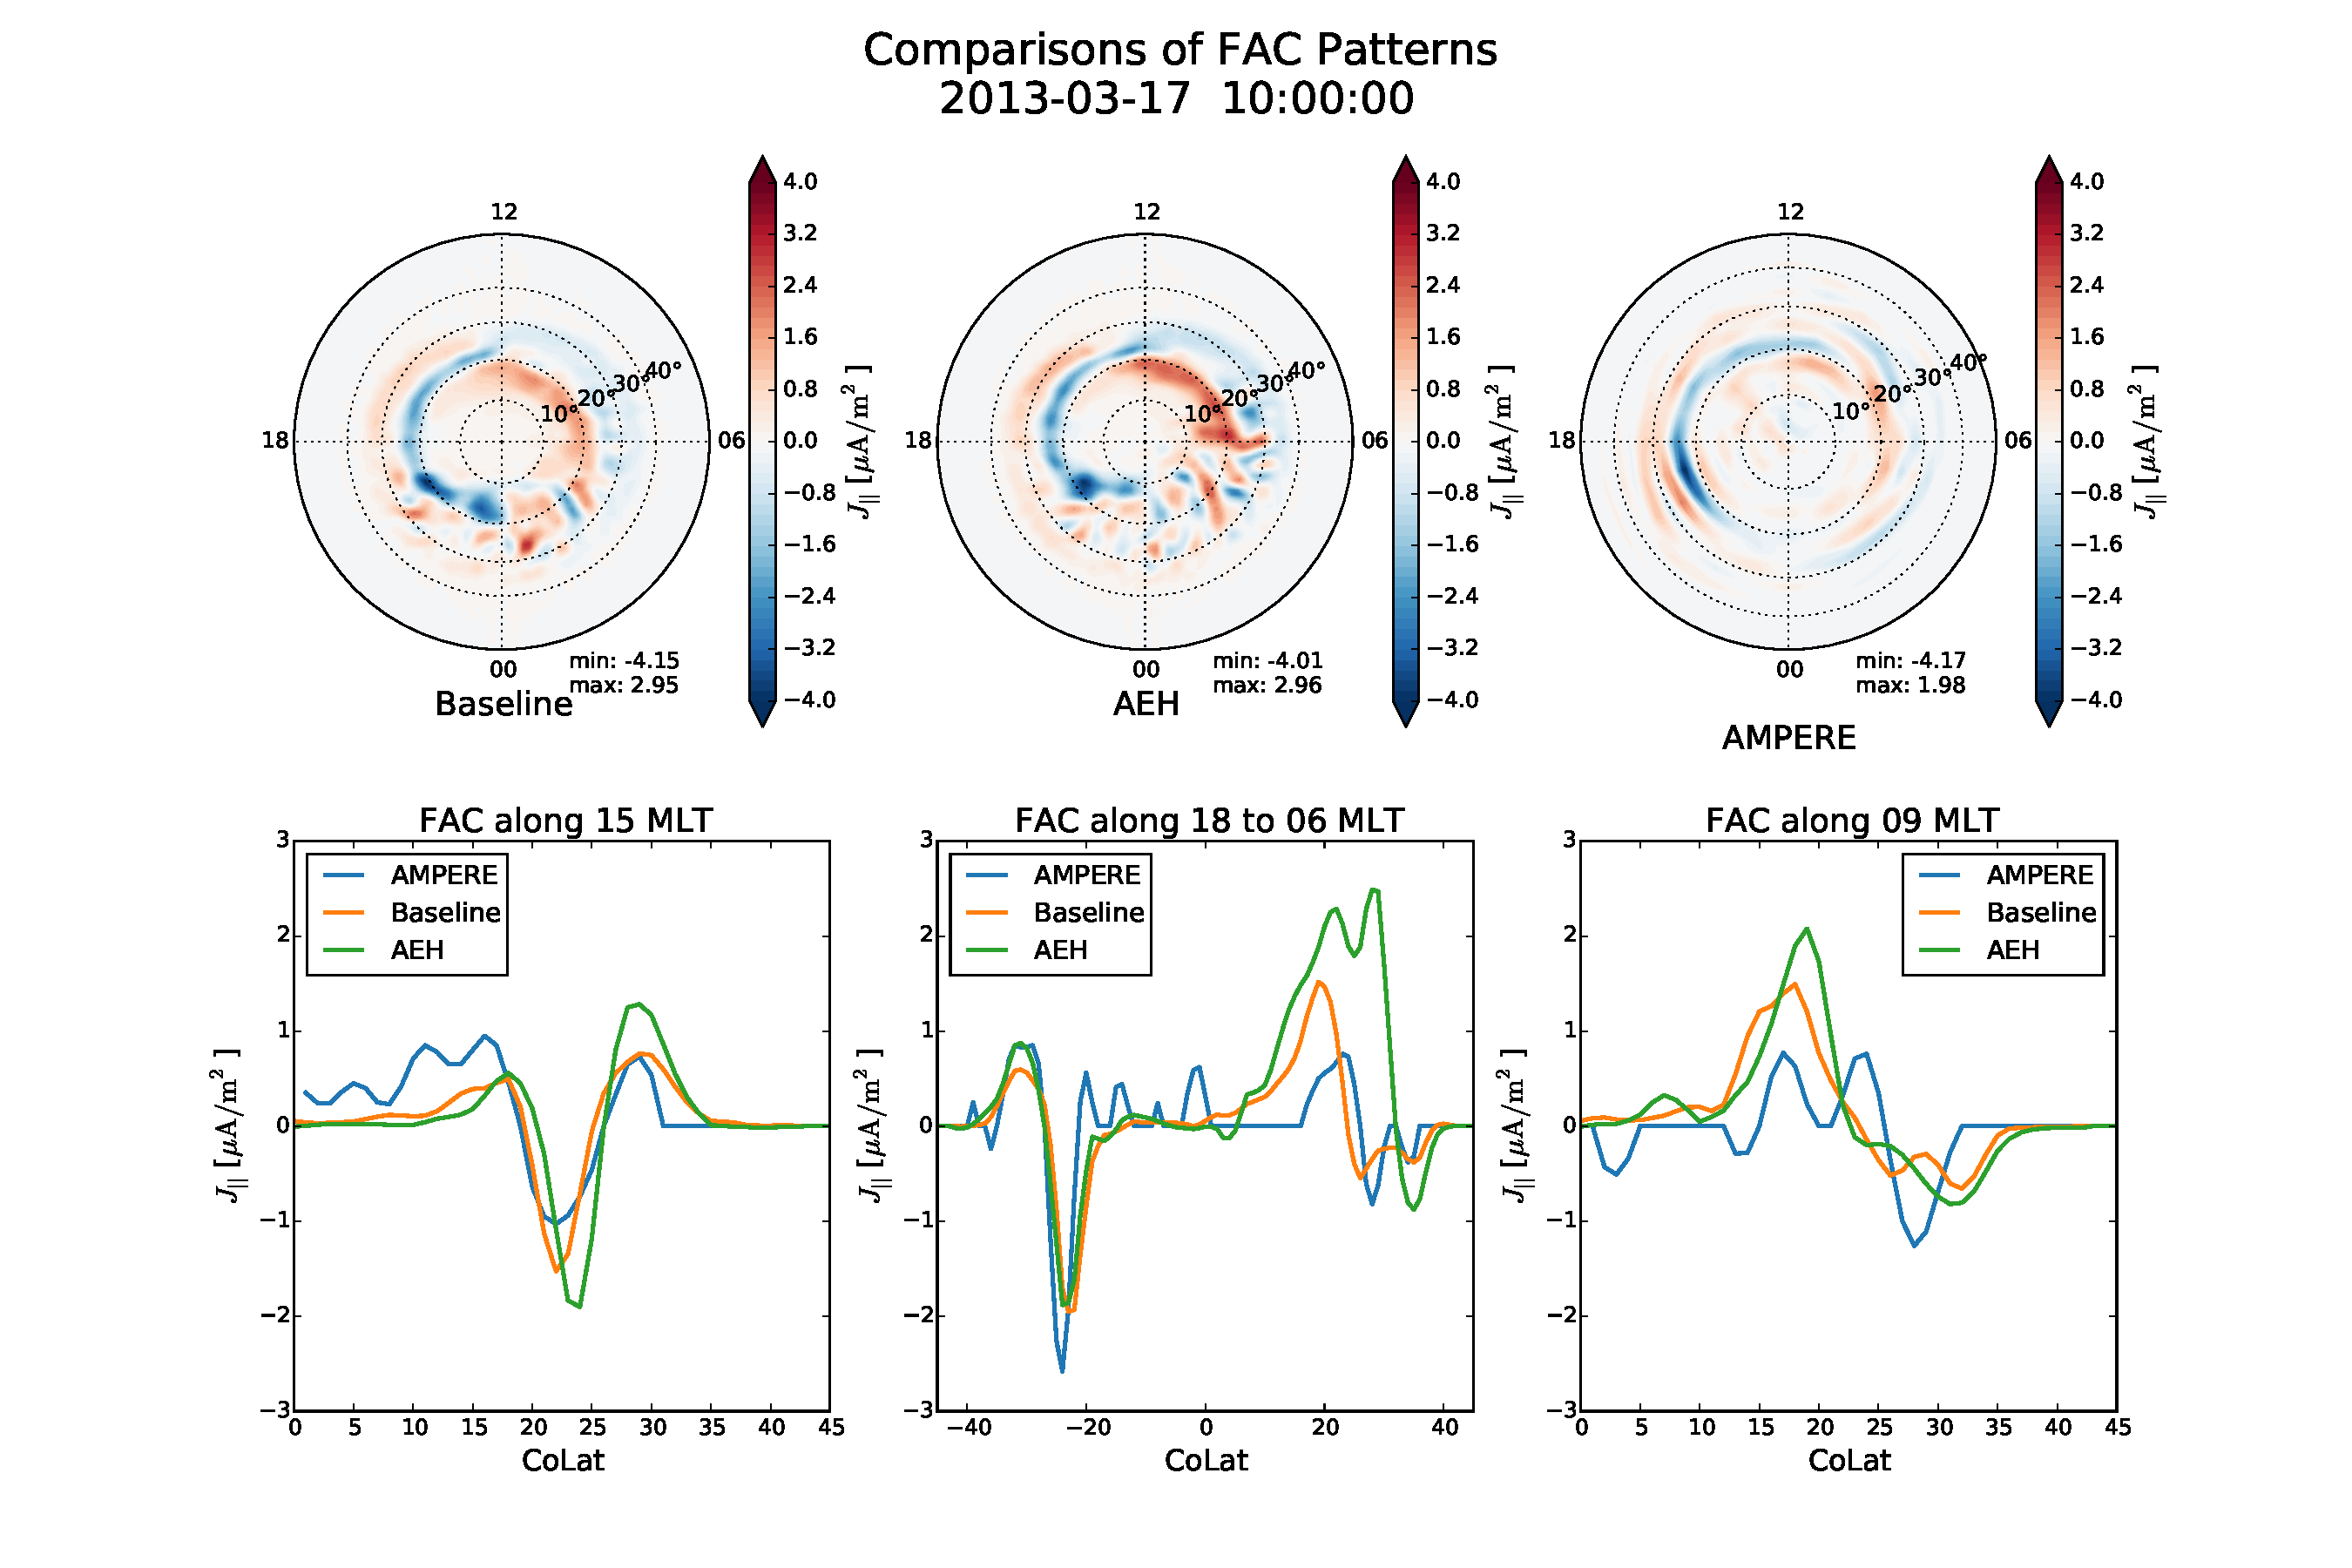
\includegraphics[width=39pc]{AmpereComparison.pdf}
\caption{\label{ampere-comp-fig}
Temporary Figure comparing AMPERE and LFM-RCM}
\end{figure*}

 \subsection{Comparison with TS07-D}
 May include a comparison with pressures in the in the ring current depending on length and quality of comparison.
 
\begin{figure*}[t]
\noindent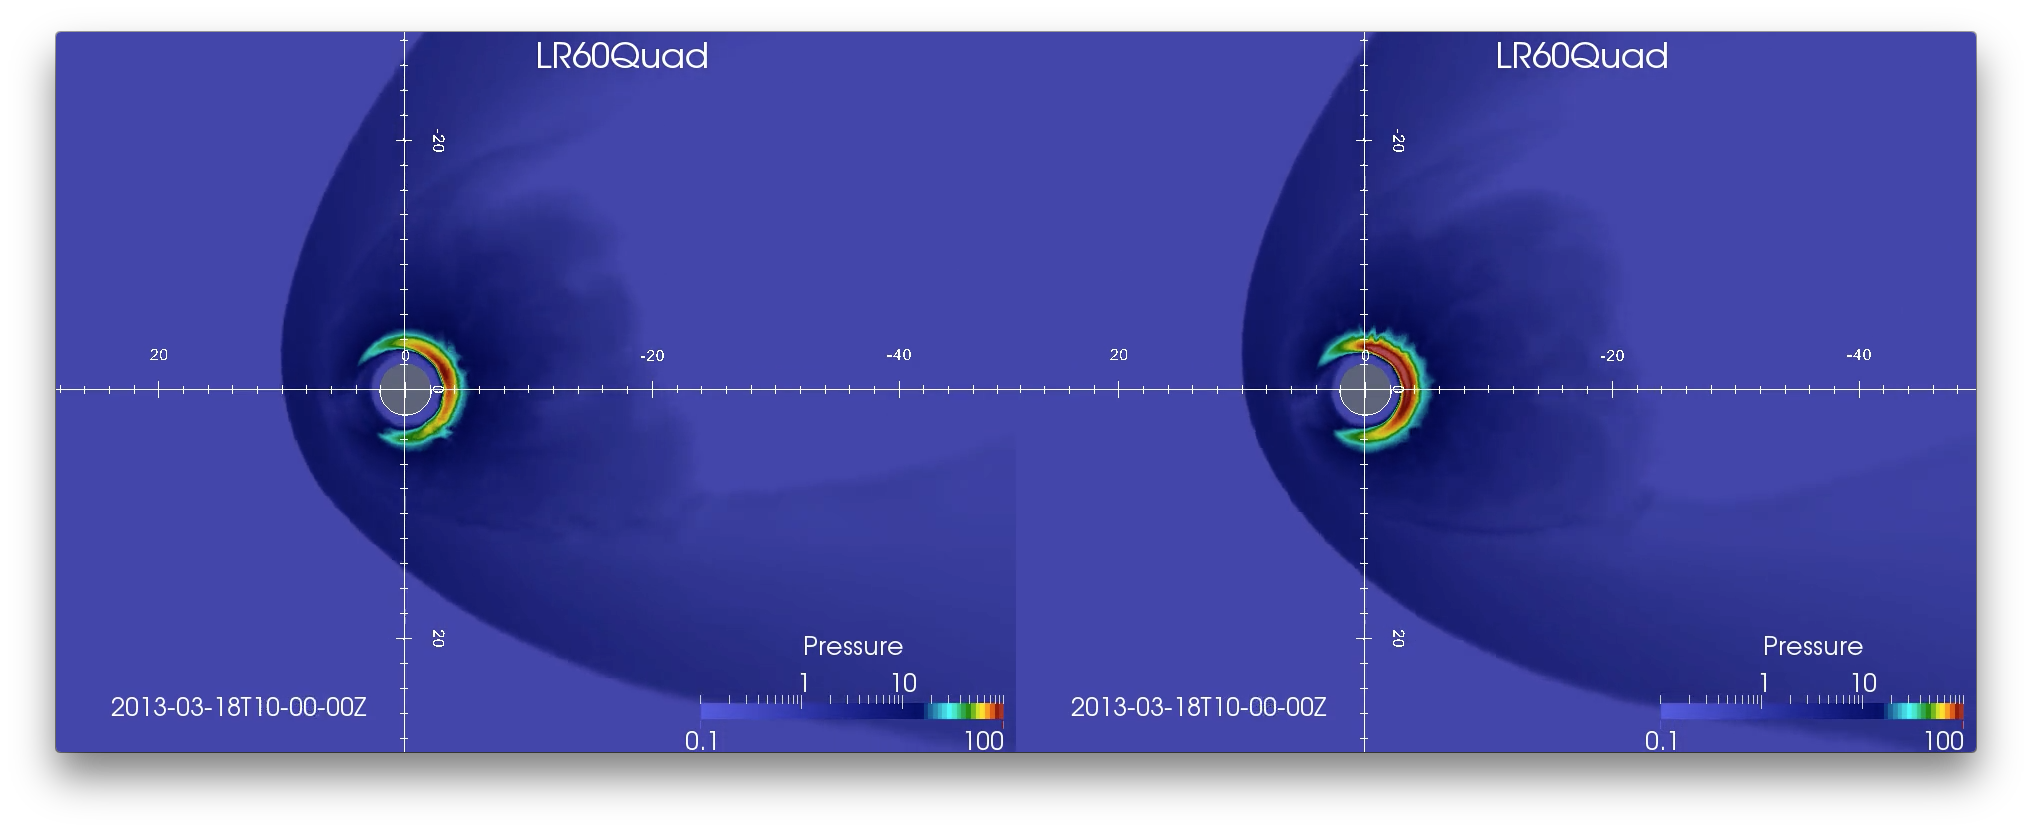
\includegraphics[width=39pc]{PressureComparison.png}
\caption{\label{press-fig}
Temporary Figure comparing Baseline and AEH pressures}
\end{figure*}


 \section{Summary and Future Directions}
\label{sec-future}

Our SAPS are the best!


%%% End of body of article:

%%%%%%%%%%%%%%%%%%%%%%%%%%%%%%%%
%% Optional Appendix goes here
%
% \appendix resets counters and redefines section heads
% but doesn't print anything.
% After typing  \appendix
%
% \section{Here Is Appendix Title}
% will show
% Appendix A: Here Is Appendix Title
%
%%%%%%%%%%%%%%%%%%%%%%%%%%%%%%%%%%%%%%%%%%%%%%%%%%%%%%%%%%%%%%%%
%
% Optional Glossary or Notation section, goes here
%
%%%%%%%%%%%%%%
% Glossary is only allowed in Reviews of Geophysics
% \section*{Glossary}
% \paragraph{Term}
% Term Definition here
%
%%%%%%%%%%%%%%
% Notation -- End each entry with a period.
% \begin{notation}
% Term & definition.\\
% Second term & second definition.\\
% \end{notation}
%%%%%%%%%%%%%%%%%%%%%%%%%%%%%%%%%%%%%%%%%%%%%%%%%%%%%%%%%%%%%%%%
%
%  ACKNOWLEDGMENTS

\begin{acknowledgments}
This material is based upon work supported by NASA grants NNX13AE39G, NNX13AF82G, NNX12AD31G, and NNX13AF78G.  The National Center for Atmospheric Research is sponsored by the National Science Foundation.  All model output, simulation codes, and analysis routines are being preserved on the NCAR High Performance Storage System and will be made available upon written request to the lead author of this publication.  The computations were performed on Kraken through an allocation of advanced computing resources provided by the Extreme Science and Engineering Discovery Environment (XSEDE), which is supported by NSF grant OCI-1053575.
\end{acknowledgments}

%% ------------------------------------------------------------------------ %%
%%  REFERENCE LIST AND TEXT CITATIONS
%
% Either type in your references using
% \begin{thebibliography}{}
% \bibitem{}
% Text
% \end{thebibliography}
%
% Or,
%
% If you use BiBTeX for your references, please use the agufull08.bst file (available at % ftp://ftp.agu.org/journals/latex/journals/Manuscript-Preparation/) to produce your .bbl
% file and copy the contents into your paper here.
%
% Follow these steps:
% 1. Run LaTeX on your LaTeX file.
%
% 2. Make sure the bibliography style appears as \bibliographystyle{agu08full}. Run BiBTeX on your LaTeX 
% file.
%
% 3. Open the new .bbl file containing the reference list and
%   copy all the contents into your LaTeX file here.
%
% 4. Comment out the old \bibliographystyle and \bibliography commands.
%
% 5. Run LaTeX on your new file before submitting.
%
% AGU does not want a .bib or a .bbl file. Please copy in the contents of your .bbl file here.

%\begin{thebibliography}{}

%\providecommand{\natexlab}[1]{#1}
%\expandafter\ifx\csname urlstyle\endcsname\relax
%  \providecommand{\doi}[1]{doi:\discretionary{}{}{}#1}\else
%  \providecommand{\doi}{doi:\discretionary{}{}{}\begingroup
%  \urlstyle{rm}\Url}\fi
%
%\bibitem[{\textit{Atkinson and Sloan}(1991)}]{AtkinsonSloan}
%Atkinson, K., and I.~Sloan (1991), The numerical solution of first-kind
%  logarithmic-kernel integral equations on smooth open arcs, \textit{Math.
%  Comp.}, \textit{56}(193), 119--139.
%
%\bibitem[{\textit{Colton and Kress}(1983)}]{ColtonKress1}
%Colton, D., and R.~Kress (1983), \textit{Integral Equation Methods in
%  Scattering Theory}, John Wiley, New York.
%
%\bibitem[{\textit{Hsiao et~al.}(1991)\textit{Hsiao, Stephan, and
%  Wendland}}]{StephanHsiao}
%Hsiao, G.~C., E.~P. Stephan, and W.~L. Wendland (1991), On the {D}irichlet
%  problem in elasticity for a domain exterior to an arc, \textit{J. Comput.
%  Appl. Math.}, \textit{34}(1), 1--19.
%
%\bibitem[{\textit{Lu and Ando}(2012)}]{LuAndo}
%Lu, P., and M.~Ando (2012), Difference of scattering geometrical optics
%  components and line integrals of currents in modified edge representation,
%  \textit{Radio Sci.}, \textit{47},  RS3007, \doi{10.1029/2011RS004899}.
%\end{thebibliography}

\bibliographystyle{agu08}
\bibliography{papers-full}
%Reference citation examples:

%...as shown by \textit{Kilby} [2008].
%...as shown by {\textit  {Lewin}} [1976], {\textit  {Carson}} [1986], {\textit  {Bartholdy and Billi}} [2002], and {\textit  {Rinaldi}} [2003].
%...has been shown [\textit{Kilby et al.}, 2008].
%...has been shown [{\textit  {Lewin}}, 1976; {\textit  {Carson}}, 1986; {\textit  {Bartholdy and Billi}}, 2002; {\textit  {Rinaldi}}, 2003].
%...has been shown [e.g., {\textit  {Lewin}}, 1976; {\textit  {Carson}}, 1986; {\textit  {Bartholdy and Billi}}, 2002; {\textit  {Rinaldi}}, 2003].

%...as shown by \citet{jskilby}.
%...as shown by \citet{lewin76}, \citet{carson86}, \citet{bartoldy02}, and \citet{rinaldi03}.
%...has been shown \citet{jskilbye}.
%...has been shown \citet{lewin76,carson86,bartoldy02,rinaldi03}.
%...has been shown \citet [e.g.,][]{lewin76,carson86,bartoldy02,rinaldi03}.
%
% Please use ONLY \citet and \citet for reference citations.
% DO NOT use other cite commands (e.g., \cite, \citeyear, \nocite, \citealp, etc.).

%% ------------------------------------------------------------------------ %%
%
%  END ARTICLE
%
%% ------------------------------------------------------------------------ %%
\newpage
\end{article}

%% Enter Figures and Tables here:

% When submitting articles through the GEMS system:
% COMMENT OUT ANY COMMANDS THAT INCLUDE GRAPHICS.
%
% DO NOT USE \psfrag or \subfigure commands.
%
% Figure captions go below the figure.
% Table titles go above tables; all other caption information
%  should be placed in footnotes below the table.

% DRAFT figure/table, including eps graphics
%
% \begin{figure}
% \noindent\includegraphics[width=20pc]{samplefigure.eps}
% \caption{Caption text here}
% \end{figure}
% \end{document}
%
% \begin{table}
% \caption{}
% \end{table}
%
% ---------------
% TWO-COLUMN figure/table
%
% \begin{figure*}
% \noindent\includegraphics[width=39pc]{samplefigure.eps}
% \caption{Caption text here}
% \end{figure*}
%
% \begin{table*}
% \caption{Caption text here}
% \end{table*}
%
% ---------------
% EXAMPLE TABLE
%
%\begin{table}
%\caption{Time of the Transition Between Phase 1 and Phase 2\tablenotemark{a}}
%\centering
%\begin{tabular}{l c}
%\hline
% Run  & Time (min)  \\
%\hline
%  $l1$  & 260   \\
%  $l2$  & 300   \\
%  $l3$  & 340   \\
%  $h1$  & 270   \\
%  $h2$  & 250   \\
%  $h3$  & 380   \\
%  $r1$  & 370   \\
%  $r2$  & 390   \\
%\hline
%\end{tabular}
%\tablenotetext{a}{Footnote text here.}
%\end{table}










% See below for how to make landscape/sideways figures or tables.

\end{document}

%%%%%%%%%%%%%%%%%%%%%%%%%%%%%%%%%%%%%%%%%%%%%%%%%%%%%%%%%%%%%%%

More Information and Advice:

%% ------------------------------------------------------------------------ %%
%
%  SECTION HEADS
%
%% ------------------------------------------------------------------------ %%

% Capitalize the first letter of each word (except for
% prepositions, conjunctions, and articles that are
% three or fewer letters).

% AGU follows standard outline style; therefore, there cannot be a section 1 without
% a section 2, or a section 2.3.1 without a section 2.3.2.
% Please make sure your section numbers are balanced.
% ---------------
% Level 1 head
%
% Use the \section{} command to identify level 1 heads;
% type the appropriate head wording between the curly
% brackets, as shown below.
%
%An example:
%\section{Level 1 Head: Introduction}
%
% ---------------
% Level 2 head
%
% Use the \subsection{} command to identify level 2 heads.
%An example:
%\subsection{Level 2 Head}
%
% ---------------
% Level 3 head
%
% Use the \subsubsection{} command to identify level 3 heads
%An example:
%\subsubsection{Level 3 Head}
%
%---------------
% Level 4 head
%
% Use the \subsubsubsection{} command to identify level 3 heads
% An example:
%\subsubsubsection{Level 4 Head} An example.
%
%% ------------------------------------------------------------------------ %%
%
%  IN-TEXT LISTS
%
%% ------------------------------------------------------------------------ %%
%
% Do not use bulleted lists; enumerated lists are okay.
% \begin{enumerate}
% \item
% \item
% \item
% \end{enumerate}
%
%% ------------------------------------------------------------------------ %%
%
%  EQUATIONS
%
%% ------------------------------------------------------------------------ %%

% Single-line equations are centered.
% Equation arrays will appear left-aligned.

Math coded inside display math mode \[ ...\]
 will not be numbered, e.g.,:
 \[ x^2=y^2 + z^2\]

 Math coded inside \begin{equation} and \end{equation} will
 be automatically numbered, e.g.,:
 \begin{equation}
 x^2=y^2 + z^2
 \end{equation}

% IF YOU HAVE MULTI-LINE EQUATIONS, PLEASE
% BREAK THE EQUATIONS INTO TWO OR MORE LINES
% OF SINGLE COLUMN WIDTH (20 pc, 8.3 cm)
% using double backslashes (\\).

% To create multiline equations, use the
% \begin{eqnarray} and \end{eqnarray} environment
% as demonstrated below.
\begin{eqnarray}
  x_{1} & = & (x - x_{0}) \cos \Theta \nonumber \\
        && + (y - y_{0}) \sin \Theta  \nonumber \\
  y_{1} & = & -(x - x_{0}) \sin \Theta \nonumber \\
        && + (y - y_{0}) \cos \Theta.
\end{eqnarray}

%If you don't want an equation number, use the star form:
%\begin{eqnarray*}...\end{eqnarray*}

% Break each line at a sign of operation
% (+, -, etc.) if possible, with the sign of operation
% on the new line.

% Indent second and subsequent lines to align with
% the first character following the equal sign on the
% first line.

% Use an \hspace{} command to insert horizontal space
% into your equation if necessary. Place an appropriate
% unit of measure between the curly braces, e.g.
% \hspace{1in}; you may have to experiment to achieve
% the correct amount of space.


%% ------------------------------------------------------------------------ %%
%
%  EQUATION NUMBERING: COUNTER
%
%% ------------------------------------------------------------------------ %%

% You may change equation numbering by resetting
% the equation counter or by explicitly numbering
% an equation.

% To explicitly number an equation, type \eqnum{}
% (with the desired number between the brackets)
% after the \begin{equation} or \begin{eqnarray}
% command.  The \eqnum{} command will affect only
% the equation it appears with; LaTeX will number
% any equations appearing later in the manuscript
% according to the equation counter.
%

% If you have a multiline equation that needs only
% one equation number, use a \nonumber command in
% front of the double backslashes (\\) as shown in
% the multiline equation above.

%% ------------------------------------------------------------------------ %%
%
%  LANDSCAPE/SIDEWAYS FIGURE AND TABLE EXAMPLES
%
%% ------------------------------------------------------------------------ %%
%
% For figures, add \usepackage{lscape} to the file and the landscape.sty style file
% to the paper folder.
%
% \begin{figure*}[p]
% \begin{landscapefigure*}
% Illustration here.
% \caption{caption here}
% \end{landscapefigure*}
% \end{figure*}
%
% For tables, add \usepackage{rotating} to the paper and add the rotating.sty file to the folder.
%
% AGU prefers the use of {sidewaystable} over {landscapetable} as it causes fewer problems.
%
% \begin{sidewaystable}
% \caption{}
% \begin{tabular}
% Table layout here.
% \end{tabular}
% \end{sidewaystable}
%
%

